\chapter{Trabalhos correlatos}
\label{cap:trabalhos-correlatos}

Neste capítulo, de maneira cronológica, serão apresentadas algumas abordagens que trataram de problemáticas análogas ao do presente trabalho, descrevendo, brevemente, suas respectivas soluções.

\section{\textit{Generalized Use of Non-Terminal Symbols for Procedural Modeling}} % LEITURAS [97]
\label{sec:paper_krekclau2010}

\citeonline{krekclau2010} utiliza deformação de forma livre como um objeto não-terminal alternativo para superar a desvantagem da criação de objetos arredondados. Para isto, é introduzida a linguagem de modelagem procedural \gls{G2}, que adapta vários conceitos de linguagens de programação de propósito geral, a fim de fornecer alto poder descritivo, com semântica bem definida, e uma sintaxe simples. 

Segundo \citeonline{krekclau2010}, o termo "\textit{generalized}" \; reflete dois tipos de generalização. Por um lado, entende-se como o escopo das linguagens de modelagem de arquitetura anteriores, permitindo vários tipos de objetos não-terminais com operadores e atributos específicos de domínio. Por outro lado, a linguagem também aceita símbolos não-terminais como parâmetros nas regras de modelagem, permitindo a definição de modelos de estrutura abstrata para reutilização dentro da gramática de maneira flexível. 

\citeonline{krekclau2010} afirmam que uma das principais características da \gls{G2} é a introdução de classes não-terminais, as quais fornecem diferentes conceitos de modelagem. Assim, as regras da Figura \ref{fig:g2_regras} devem ser de um tipo específico, uma vez que os operadores de cada regra só podem ser aplicados a um determinado tipo de objeto não-terminal. Por exemplo, a classe não-terminal \textit{Box} se comporta de maneira semelhante à \textit{CGA Shape}, fornecendo transformações simples, bem como operadores de repetição e divisão para um objeto da cena. Além disto, as deformações de forma livre fornecem operadores para manipular os pontos de controle deste objeto. Todas as classes possuem atributos declarados implicitamente, os quais descrevem o objeto não-terminal. Uma \textit{Box}, por exemplo, tem os três atributos $size_x$, $size_y$ e $size_z$, enquanto uma deformação de forma livre armazena as posições 3D de todos os seus pontos de controle $c_{xyz}$ com $x, y, z \in \{0, 1\}$. Tais atributos podem ser, então, utilizados para realização de cálculos adicionais, conforme ilustrado na Figura \ref{fig:g2_regras}, onde a regra \texttt{C} fornece uma declaração de parâmetro explícita, enquanto a regra \texttt{A} utiliza o parâmetro implícito $size_x$ do objeto não-terminal \textit{Box}, que contém a largura atual.

\begin{figure}[h!]
	\centering
	\captionsetup{width=15cm}
	\Caption{\label{fig:g2_regras} Aplicação de regras de modelagem da \gls{G2}.}	
	\UFCfig{}{
		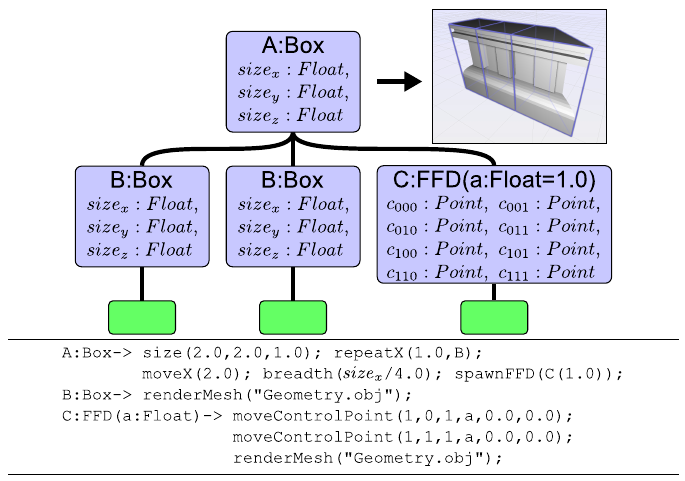
\includegraphics[width=13cm]{figuras/g2_rules.png}
	}
	{\Fonte{\cite{krekclau2010}}}	
\end{figure}

\newpage

Para ilustrar a utilização da \gls{G2} na geração de estruturas arredondadas, \citeonline{krekclau2010} apresentam alguns exemplos. Na Figura \ref{fig:g2_exemplo_1} é mostrado um caso típico de beirais passando ao redor de uma borda. Na segunda imagem, uma nova geometria deve ser carregada para cobrir a região afiada. A terceira imagem mostra que deformações de forma livre resolvem o problema, e que a geometria utilizada para o beiral ao longo da parede pode ser reutilizada para o canto. A Figura \ref{fig:g2_exemplo_2}, por sua vez, mostra a criação de bordas arredondadas após a aplicação de múltiplas deformações.

\begin{figure}[h!]
	\centering
	\captionsetup{width=15cm}
	\Caption{\label{fig:g2_exemplo_1} Exemplo típico de beirais passando ao redor de uma borda.}	
	\UFCfig{}{
		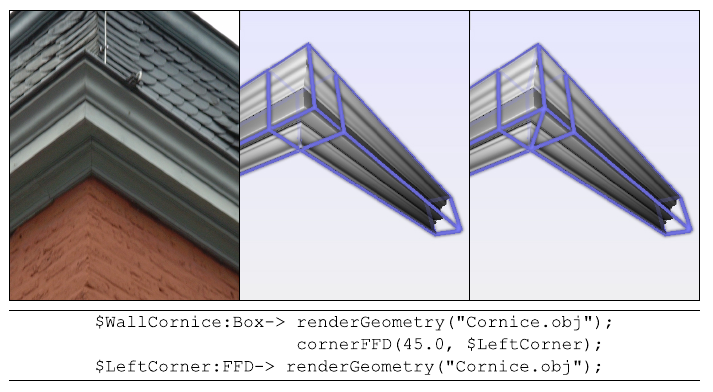
\includegraphics[width=15cm]{figuras/g2_round_1.png}
	}
	{\Fonte{\cite{krekclau2010}}}	
\end{figure}

\begin{figure}[h!]
	\centering
	\captionsetup{width=15cm}
	\Caption{\label{fig:g2_exemplo_2} Aplicação de sucessivas deformações de forma livre através da \gls{G2}.}	
	\UFCfig{}{
		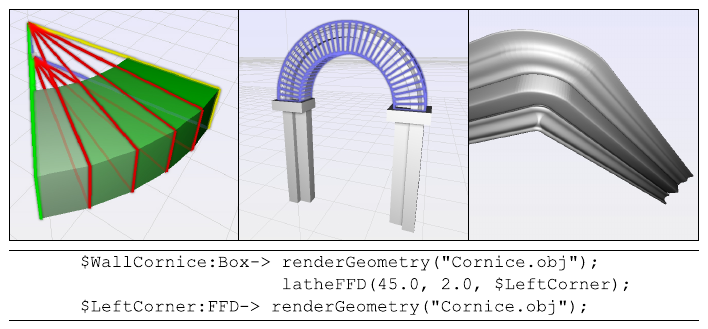
\includegraphics[width=15cm]{figuras/g2_round_2.png}
	}
	{\Fonte{\cite{krekclau2010}}}	
\end{figure}

Como limitação da \gls{G2}, \citeonline{krekclau2010} apontam a incapacidade da realização de consultas geométricas, algo que é possível na \textit{CGA Shape}, por exemplo. Além disto, também percebeu-se que as deformações desta abordagem são utilizadas apenas para geração de ornamentos arredondados, como os beirais da Figura \ref{fig:g2_exemplo_1}, ou seja, não são aplicadas especificamente para geração de modelos de massa com geometria arredondada.

\newpage
\clearpage

\section{\textit{Procedural architecture using deformation-aware split grammars}} % LEITURAS [90]
\label{sec:paper_zmugg2014_sec1}

Uma extensão às \textit{split grammars} é apresentada por \citeonline{zmugg2014}, permitindo a criação de arquiteturas curvadas através da integração de deformações de forma livre em qualquer nível de uma gramática. 

\citeonline{zmugg2014} afirmam que, geralmente, regras de divisão são realizadas de duas maneiras diferentes, ou podendo se adaptar às deformações, para que as repetições possam se ajustar a mais ou menos espaço, mantendo as restrições de comprimento; ou podem dividir a geometria deformada com planos, a fim de introduzir estruturas retas na geometria deformada.

De acordo com \citeonline{zmugg2014}, existem muitos edifícios e estruturas que podem ser entendidos como tendo uma forma reta, mas que, em algum momento, é distorcida para uma forma curvada. Um exemplo ilustrativo é mostrado na Figura \ref{fig:field_wall}, onde uma grande parede de pedra se estende por uma paisagem.

\begin{figure}[h!]
	\centering
	\captionsetup{width=15cm}
	\Caption{\label{fig:field_wall} Muralha que se estende em um terreno.}	
	\UFCfig{}{
		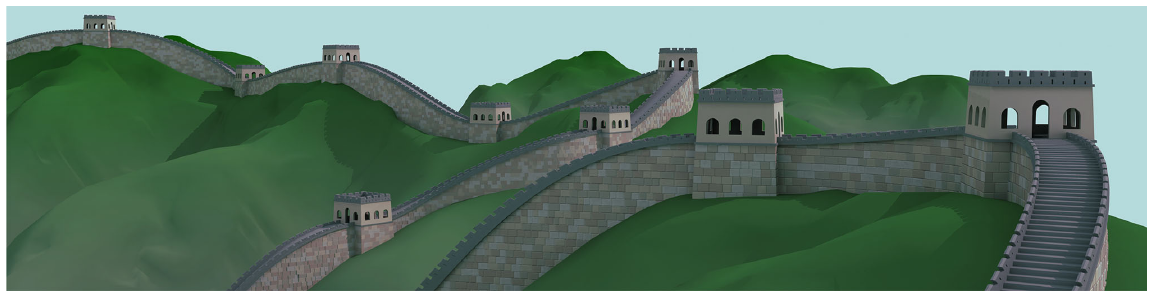
\includegraphics[width=15cm]{figuras/field.png}
	}
	{\Fonte{\cite{zmugg2014}}}	
\end{figure}

\subsection{Integrando deformações de forma livre}
\label{sec:zmugg2014_sec3}

Segundo \citeonline{zmugg2014}, para integrar as deformações de forma livre em sua abordagem, substituiu-se a transformação rígida, utilizada em \textit{split grammars} tradicionais, por uma lista de deformações arbitrárias, o que permite a aplicação aninhada de deformações de forma livre. Este processo é mostrado na Figura \ref{fig:zmugg_ffd}, onde, a partir de uma forma simples representando uma parede (a), são aplicadas três etapas de deformação: primeiro, apenas a base amarela é afetada pela deformação de alargamento (b), logo após, são aplicadas as deformações verticais (c) e horizontais (d).

\begin{figure}[h!]
	\centering
	\captionsetup{width=15cm}
	\Caption{\label{fig:zmugg_ffd} Aplicação aninhada de deformações de forma livre em uma \textit{split grammar}.}	
	\UFCfig{}{
		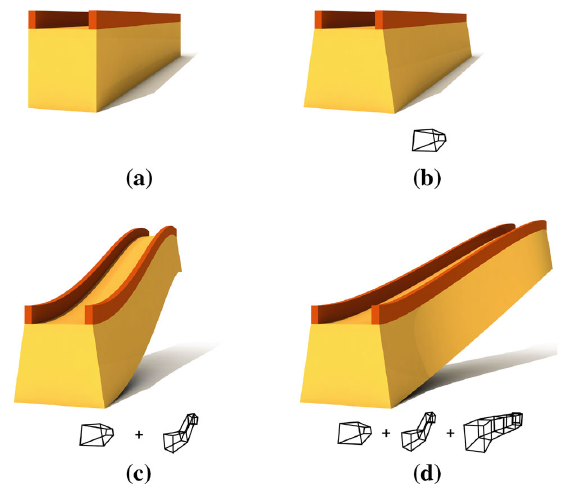
\includegraphics[width=12cm]{figuras/zmugg_ffd.png}
	}
	{\Fonte{\cite{zmugg2014}}}	
\end{figure}

\newpage

Com objetivo de demonstrar a utilização das regras de deformação em um modelo geométrico, \citeonline{zmugg2014} apresentam o exemplo da Figura \ref{fig:zmugg_rules}. Nas regras mostradas na região inferior, o rótulo \textit{Box} refere-se a uma caixa ainda não deformada, representada na Figura \ref{fig:zmugg_rules}(a). A operação \texttt{deform} recebe como entrada a caixa delimitadora em coordenadas locais, o número de pontos de controle na direção dos eixos $x$, $y$ e $z$, bem como uma matriz de deslocamento individual para cada um destes pontos de controle. Algumas funções utilitárias podem ser definidas para permitir uma especificação mais conveniente de deformações comuns. Assim, depois de definir a deformação, pode-se utilizar as operações de divisão padrão, como \texttt{divide}, ou novas operações de divisão, que são indicadas pelo sufixo \texttt{D}. Entretanto, para utilização de novas operações, é necessário fornecer um ponto adicional como entrada, o qual, juntamente com a direção em que a divisão deve ocorrer, é utilizado para calcular a distância entre os dois extremos no espaço deformado. Por fim, a operação de preenchimento renderiza as formas com o material definido para o atributo \textit{mat}, resultando na Figura \ref{fig:zmugg_rules}(b).

\begin{figure}[h!]
	\centering
	\captionsetup{width=15cm}
	\Caption{\label{fig:zmugg_rules} Aplicação de regras de subdivisão em objetos.}	
	\UFCfig{}{
		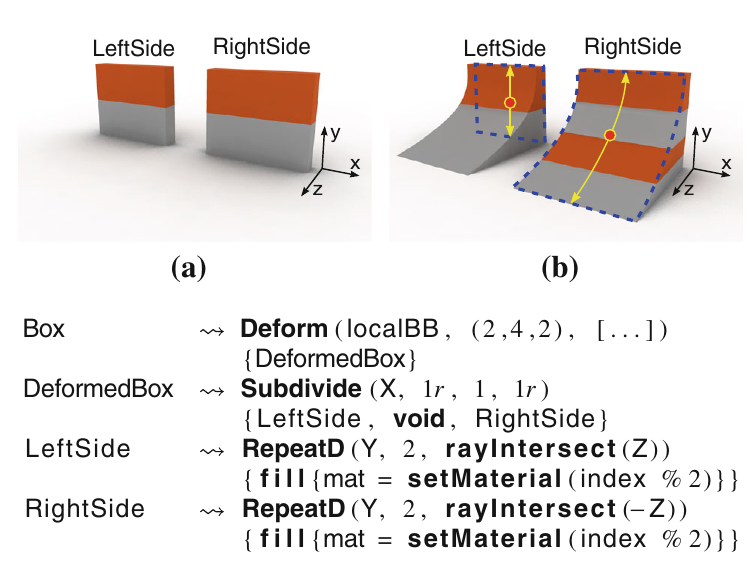
\includegraphics[width=12cm]{figuras/havemann_model_rules.png}
	}
	{\Fonte{Adaptado de \cite{zmugg2014}}}	
\end{figure}

\newpage

Por meio do exemplo mostrado na Figura \ref{fig:facade_curve}, \citeonline{zmugg2014} demonstram o efeito das operações de deformação em um modelo de fachada. As divisões ao longo da largura da fachada são feitas em relação à deformação. Para lidar com o espaço adicional fornecido pela deformação, mais divisões são introduzidas no espaço de coordenadas local, conforme ilustrado na Figura \ref{fig:facade_curve}(c).

\begin{figure}[h!]
	\centering
	\captionsetup{width=15cm}
	\Caption{\label{fig:facade_curve} A aplicação de deformações em uma fachada reta, que é definida utilizando uma \textit{split grammar} (a), produz um número diferente de janelas nas partes laterais (b). A imagem inferior (c) mostra as divisões que são realizadas no espaço de coordenadas locais (não deformadas) para alcançar o resultado mostrado após a deformação (b).}	
	\UFCfig{}{
		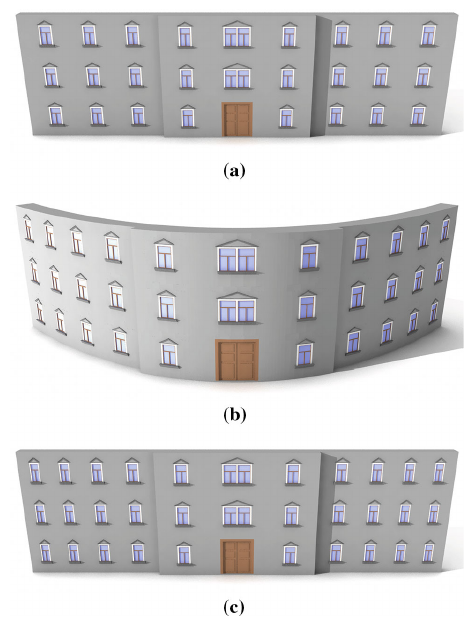
\includegraphics[width=13cm]{figuras/facade_curve.png}
	}
	{\Fonte{\cite{zmugg2014}}}	
\end{figure}

\subsection{Aplicações}
\label{sec:zmugg2014_sec5}

Um dos resultados apresentados por \citeonline{zmugg2014} é o de um edifício oblongo que é dobrado de diferentes maneiras, através de deformações que se aproximam de formas circulares, conforme ilustrado na Figura \ref{fig:offices}. Neste exemplo, um edifício com \textit{layout} de sala, definido utilizando uma abordagem de \textit{split grammar} (a), se adapta de acordo com diferentes deformações que se aproximam de segmentos de círculo, ou círculos. A deformação do segmento de círculo (b) leva a uma construção como mostrado em (a). Para mudanças topológicas (c), as regras gramaticais para as paredes de contorno à esquerda e à direita de (a) foram adaptadas, e uma deformação apropriada foi aplicada para alcançar uma transição contínua.

\begin{figure}[h!]
	\centering
	\captionsetup{width=15cm}
	\Caption{\label{fig:offices} Prédio comercial com estrutura arredondada.}	
	\UFCfig{}{
		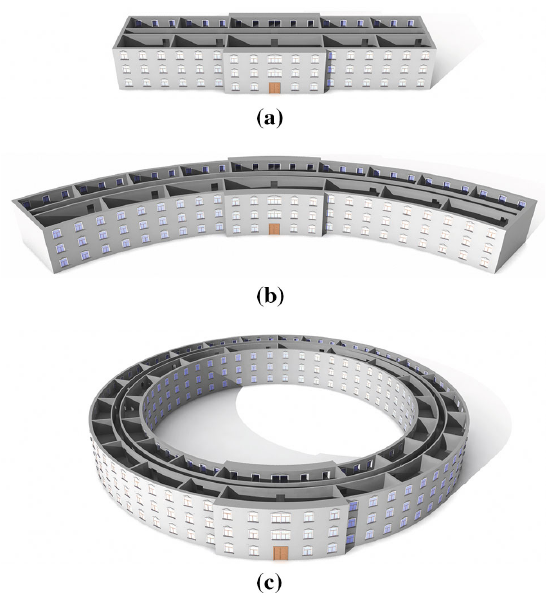
\includegraphics[width=15cm]{figuras/office_buildings_zmugg.png}
	}
	{\Fonte{\cite{zmugg2014}}}	
\end{figure}

Além da geração de modelos arquiteturais com geometria arredondada, outra vantagem relevante identificada nesta abordagem é o processo de adaptação dos elementos, como janelas e portas, após uma operação de deformação. Por exemplo, na Figura \ref{fig:facade_curve}, após alteração da curvatura da fachada, é importante notar que as janelas não são alargadas, mas sim adicionadas, a fim de se utilizar o espaço extra gerado pela deformação, todas elas possuindo a mesma largura.

Como limitação, \citeonline{zmugg2014} mencionam que seu sistema não permite que regras adaptem o resultado de operações \textit{booleanas} de elementos adjacentes.

\newpage
\clearpage

\section{\textit{Procedural modeling of architecture with round geometry}}
\label{sec:paper_edelsbrunner2017} % LEITURAS [54]

Diferentemente das abordagens apresentadas por \citeonline{fellner2013} e \citeonline{zmugg2014}, no trabalho de \citeonline{edelsbrunner2017} são especificados sistemas de coordenadas personalizados na \textit{split grammar} definida pelo usuário. Os sistemas de coordenadas cilíndricas produzem geometria adequada para modelar estruturas como torres ou pilares. Sistemas de coordenadas esféricas podem ser utilizados para domos. Além disto, outros sistemas de coordenadas também são convenientes, por exemplo, para geração de estruturas em forma de cone, podendo ser aplicadas na geração de telhados.

Apesar de não apresentarem muitos exemplos práticos da utilização de regras para geração dos modelos apresentados, \citeonline{edelsbrunner2017} afirmam que a especificação do sistema de coordenadas permite mais possibilidades na divisão de geometria. Uma divisão de parede com uma \textit{split grammar} tradicional produz partes retangulares, assim, a partir de outros sistemas de coordenadas, também é possível dividir paredes cilíndricas ou esféricas em subpartes, conforme ilustrado na Figura \ref{fig:round_geometry}.

\begin{figure}[h!]
	\centering
	\captionsetup{width=15cm}
	\Caption{\label{fig:round_geometry} Uma parede dividida em nove partes, por meio de diferentes sistemas de coordenadas (cartesiana, cilíndrica e esférica).}	
	\UFCfig{}{
		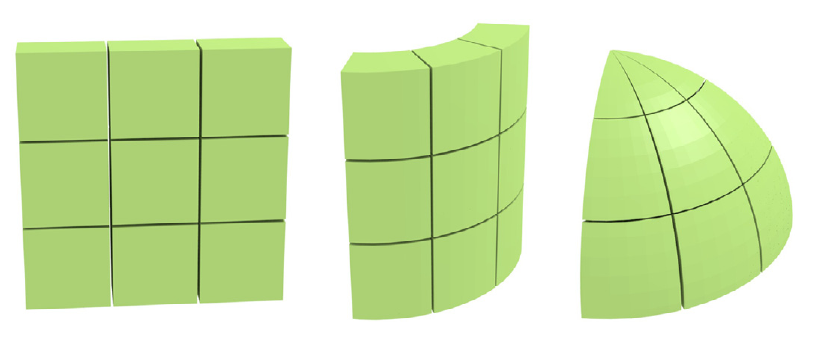
\includegraphics[width=15cm]{figuras/round_geometry.png}
	}
	{\Fonte{\cite{edelsbrunner2017}}}	
\end{figure}

Além de permitir a utilização de diferentes tipos de sistemas de coordenadas para geração dos modelos, outro recurso interessante identificado nesta abordagem é a possibilidade do usuário especificar entradas em alto nível, a fim de organizar os elementos gerados proceduralmente. Isto permite que até mesmo usuários inexperientes modifiquem o modelo e criem diferentes variações, mas sem se aprofundar em grandes detalhamentos \cite{edelsbrunner2017}, conforme os exemplos da Figura \ref{fig:vault}.

\begin{figure}[h!]
	\centering
	\captionsetup{width=15cm}
	\Caption{\label{fig:vault} Variações de modelos de abóbodas.}	
	\UFCfig{}{
		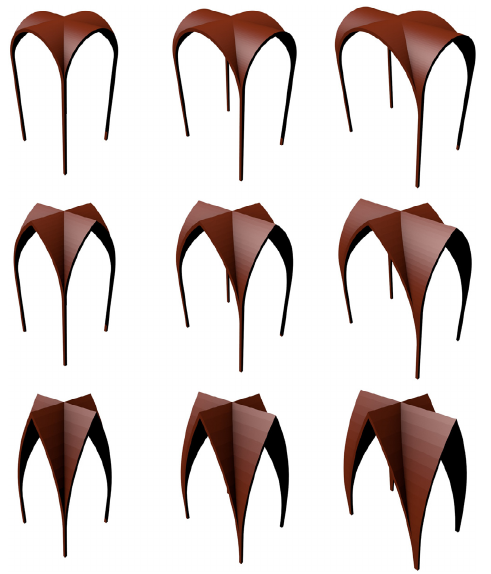
\includegraphics[width=11cm]{figuras/vault.png}
	}
	{\Fonte{\cite{edelsbrunner2017}}}	
\end{figure}

Como limitação, \citeonline{edelsbrunner2017} argumentam que objetos produzidos por meio de deformações de forma livre, que não seguem a geometria das seções cônicas, podem ser difíceis ou impossíveis de reproduzir através da sua abordagem, podendo requerer métodos de aproximação mais complexos.

\section{Considerações finais}
\label{sec:consideracoes_capitulo_3}

Neste capítulo, foram apresentadas três técnicas distintas, cada uma voltada para determinada área da geração procedural de modelos com estruturas arredondadas. No próximo capítulo, será discutido o problema abordado pelo presente trabalho, bem como a descrição de uma estratégia para resolvê-lo.
 